\section{Zielsetzung}

In diesem Versuch wird zunächst das Verhalten von einem Elektronenstrahl im elektrischen
Feld untersucht und daraufhin das Verhalten in einem transversalen Magnetfeld.

\section{Theorie}

\subsection{Elektronenstrahl im elektrischen Feld}

Die Ablenkung eines Elektronenstrahls im elektrischen Feld kann mit einer
Kathodenstrahlröhre durchgeführt werden. Der schematische Aufbau dieser ist in
Abbildung \ref{abb:1} dargestellt. Die Kathodenstrahlröhre ist evakuiert, da sonst
die Elektronen mit den Luftmolekülen Wechselwirken würden.

\begin{figure}[H]
  \centering
  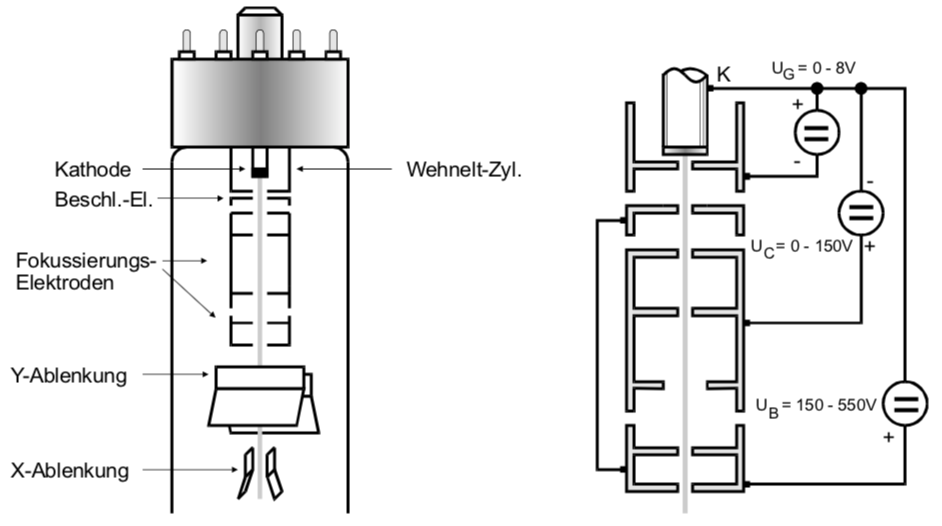
\includegraphics[width=\textwidth]{content/Kathode.png}
  \caption{Schematische Darstellung einer Kathodenstrahlröhre \cite{1}.}
  \label{abb:1}
\end{figure}

Die Kathodenstrahlröhre besteht aus drei Teilen.
Im ersten Teil werden die Elektronen durch Glühemission einer Kathode erzeugt.
Diese Kathode ist von einem Wehnelt-Zylinder umgeben, an dem eine Gegenspannung
der Kathode gegenüber anliegt. Durch diese Spannung kann die Intensität des Elektronenstrahls
eingestellt werden. Daraufhin folgt eine starke Beschleunigungsspannung $U_B$. Während
der Beschleunigung wird durch inhomogene elektrische Felder der Elektronenstrahl fokussiert.
Die Geschwindigkeit $v_z$, auf welche die Elektronen beschleunigt werden lässt sich aus dem
Energiesatz herleiten

\begin{equation*}
  \frac{m_0 v_z^2}{2} = e_0 U_b.
\end{equation*}

Dabei ist $m_0$ die Elektronenmasse und $e_0$ die Elementarladung.

In dem zweiten Teil befindet sich das Ablenksystem für den Elektronenstrahl. Dieses
besteht aus zwei senkrecht zueinander stehenden Kondensatoren. Damit kann der Elektronenstrahl
in zwei Richtungen abgelenkt werden.
Als letztes folgt ein Leuchtschirm, der an dem Auftreffpunkt des Elektronenstrahls
leuchtet.

Nun wird ein Zusammenhang zwischen der Verschiebung $D$ auf dem Schirm und der
Ablenkspannung $U_d$ hergeleitet. Dazu werden die in Abbildung \ref{abb:2} angegebenen
Bezeichnungen verwendet.

\begin{figure}[H]
  \centering
  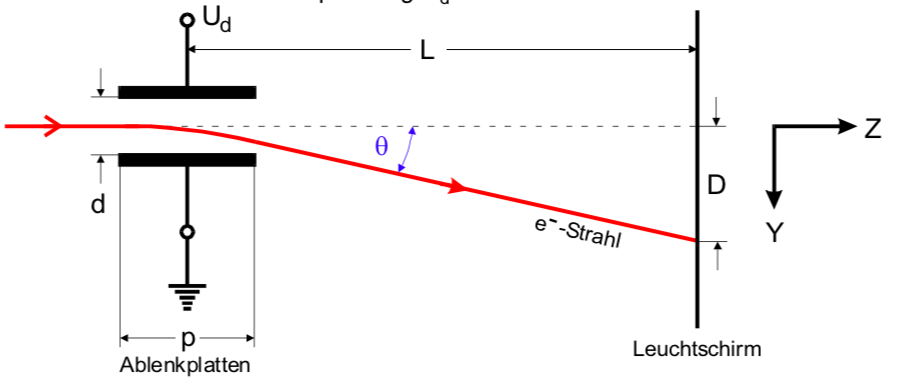
\includegraphics[width=\textwidth]{content/Ablenkung.png}
  \caption{Skizze des Ablenkvorganges in einer Kathodenstrahlröhre \cite{1}.}
  \label{abb:2}
\end{figure}

Mithilfe geometrischer Überlegungen dann der Zusammenhang

\begin{equation}
  D = \frac{p}{2d} L \frac{U_d}{U_B}.
  \label{eq:1}
\end{equation}

Mit einer Kathodenstrahlröhre kann außerdem ein Oszillograph realisiert werden,
der eine Zeitabhängige Wechselspannung darstellen kann. Dazu wird an das Plattenpaar,
welches für die horizontale Ablenkung verantwortlich ist, eine Sägezahnspannung angeschlossen.
Diese steigt mit der Zeit an und springt bei einem Maximalwert wieder auf den Anfangswert
zurück. An das andere Plattenpaar wird dann die zu untersuchende Wechselspannung angeschlossen.
Damit der zeitliche Verlauf der Wechselspannung dargestellt werden kann müssen die
Frequenzen der beiden Spannungen die Synchronisationsbedingung erfüllen

\begin{equation}
  n \nu_\text{Sä} = m \nu_\text{We} \,\,\,\,\, \text{mit} \, \, \, n=1, 2, 3, ... \, \, \, m=1, 2, 3, ...
  \label{eq:2}
\end{equation}


\subsection{Elektronenstrahl im transversalen Magnetfeld}

Auf eine Ladung $q$ in homogenen Magnetfeldern $\vec{B}$ wirkt die Lorentz-Kraft

\begin{equation*}
  \vec{F_L} = q \vec{v} \times \vec{B}.
\end{equation*}

Dabei ist $\vec{v}$ die Geschwindigkeit der Ladung. Ein Magnetfeld lenkt eine Ladung
also ab, allerdings wird an der Ladung keine Arbeit verrichtet. Das bedeutet, dass
$\vert{\vec{v}}$ konstant bleibt und somit bewegt sich die Ladung auf einer Kreisbahn im Magnetfeld,
wenn sie senkrecht in das Magnetfeld eindringt.

Mithilfe einer Kathodenstrahlröhre und einem homogenen Magnetfeld lässt sich nun die
spezifische Ladung von Elektronen $\frac{e_0}{m_0}$ bestimmen. Der Zusammenhang zwischen
Ablenkung $D$ und spezifische Ladung der Elektronen ergibt sich zu

\begin{equation}
  \frac{D}{L^2 + D^2} = \frac{1}{\sqrt{8 U_B}} \sqrt{\frac{e_0}{m_0}} B.
  \label{eq:3}
\end{equation}

Die Bezeichnungen sind dabei analog zu dem ersten Teil.
